\section{"1" Определение геометрических свойств поверхности}

\begin{frame}[t]{Определение геометрических свойств}
\framesubtitle{}
    \begin{columns}[T,onlytextwidth]
        \begin{column}{0.69\textwidth}
            \small
            С помощью \textbf{ощупывания роботом поверхности} получить \underline{плотное облако точек} и \underline{полигональную сетку}.

            \textbf{Метод решения}: Триангуляция Делоне с использованием альфа формы

            \textbf{Алгоритм}: Решив задачу локализации, получить облако точек следовой дорожки. \textbf{Очистить шумное облако точек} и его \textbf{усреднить} с помощью Voxel Grid. Применить \underline{триангуляцию Делоне для вогнутых оболочек}, получив полигональную сетку. \underline{Сгенерировать новые точки} из полигональной сетки с нужным разрешением.

            \textbf{Входные данные}: следовая дорожка, в виде облака точек.
            
            \textbf{Выходные данные}: полигональная сетка и плотное облако точек
            
            \textbf{Допустимая точность}: 0.1 м, оценки Cloud2Cloud и Cloud2Mesh

            \textbf{Предположения}: 1) Имеется поверхность. Координаты задаются $z=f(x,y)$. 2) Расстояние между ногами робота мало относительно размеров поверхности, следовательно, поверхность между ногами считается плоскостью.   
        \end{column}
        \begin{column}{0.29\textwidth}
            \begin{figure}[H]
                \begin{subfigure}{0.99\textwidth}
                    \centering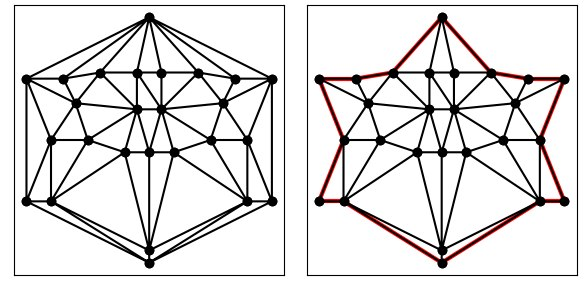
\includegraphics[height=2.5cm,width=1\textwidth,keepaspectratio]{../images/slides/delone_mag.png}
                    \caption*{Триангуляция Делоне}
                \end{subfigure}

                \begin{subfigure}{0.99\textwidth}
                    \centering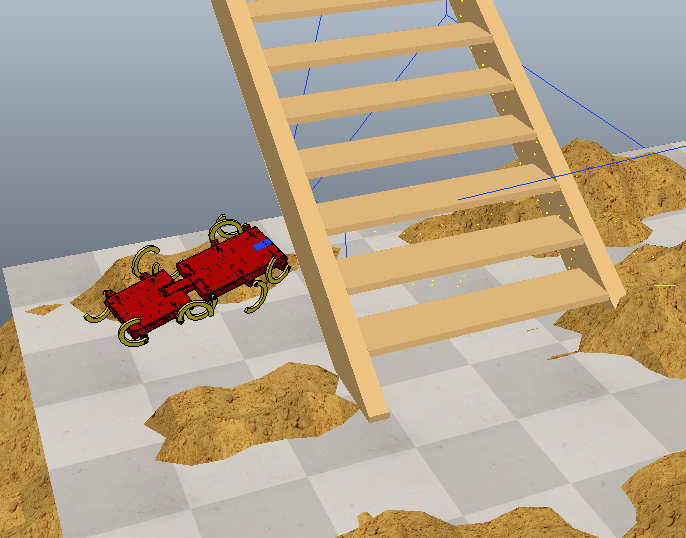
\includegraphics[height=2.5cm,width=1\textwidth,keepaspectratio]{../images/slides/error.png}
                    \caption*{Когда $z\neq f(x,y)$}
                \end{subfigure}
            \end{figure}
        \end{column}
    \end{columns}
\end{frame}

\note{\small \setlength{\parindent}{20pt}

Решив задачу 3 и 4, также возможно стало решить и задачу по определению рельефа пройденной поверхности. Необходимо с помощью ощупывания роботом поверхности получить плотное облако точек и полигональную сетку.

Для упрощения решения задачи я ввел два предположения. Во первых, у нас существуют поверхности, только где координата z уникальна для каждой пары координат x,y. Пример обратного предположения --- место под лестницей на картинке *тык*.

Второе предположение -- расстояние между ногами робота мало относительно размеров поверхности. Поэтому эта поверхность будет считаться плоскостью. Вокруг этого предположения и строится весь алгоритм.

Решив задачу локализации, о которой будет далее, мы знаем шумное облако точек следовой дорожки. Очистив и усреднив это облако точек, я применяю триангуляцию Делоне для вогнутых оболочек *тык*, тем самым получая полигональную сетку. Из полигональной сетки генерируется плотное облако точек с нужным разрешением.
}

\begin{frame}[t]{Оценки C2C и C2M}
\framesubtitle{}
    \begin{figure}[H]
        \begin{subfigure}[t]{0.49\textwidth}
            \centering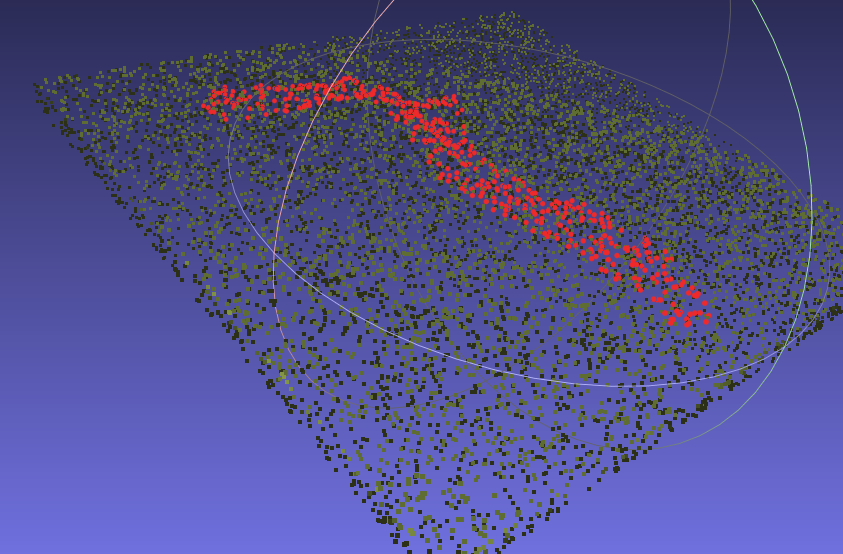
\includegraphics[height=4.5cm,width=1\textwidth,keepaspectratio]{../images/slides/c2c.png}
            \caption*{Cloud to Cloud: высчитывается абсолютное расстояние до ближайшей соседней точки}
        \end{subfigure}
        \begin{subfigure}[t]{0.49\textwidth}
            \centering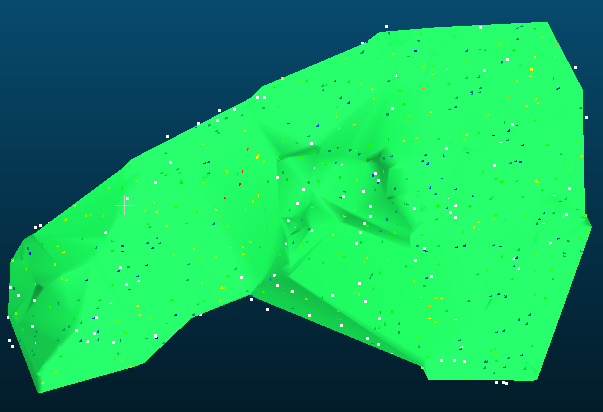
\includegraphics[height=4.5cm,width=1\textwidth,keepaspectratio]{../images/slides/c2m.png}
            \caption*{Cloud to Mesh: высчитывается расстояние с учетом знания о векторе нормали плоскости}
        \end{subfigure}
    \end{figure}
\end{frame}

\note{\small \setlength{\parindent}{20pt}

Выбор максимальной допустимой точности является нетривиальной задачей. Так как во первых, ошибка сильно зависит от сложности территории и ее размеров. Более того, возникает вопрос как считать эту ошибку. 

Мной было решено, что среднеквадратичная ошбика в 0.1 метр для пещер длиной в километр является приемлемой, так как данный метод нужен для предварительной оценки поверхности.

Критериями оценки были выбраны 2 подхода Cloud2Cloud и Cloud2Mesh. Это стандартные метрики для сравнения облаков точек в программных продуктах.

Идея в том, что С2С *тык* использует абсолютное расстояние до ближайшей соседней точки, а C2M *тык* учитывает еще в каком направлении идет отклонение от полигональной сетки.}

\begin{frame}[t]{Эксперименты}
    \begin{figure}[H]
        \begin{subfigure}[t]{0.49\textwidth}
            \centering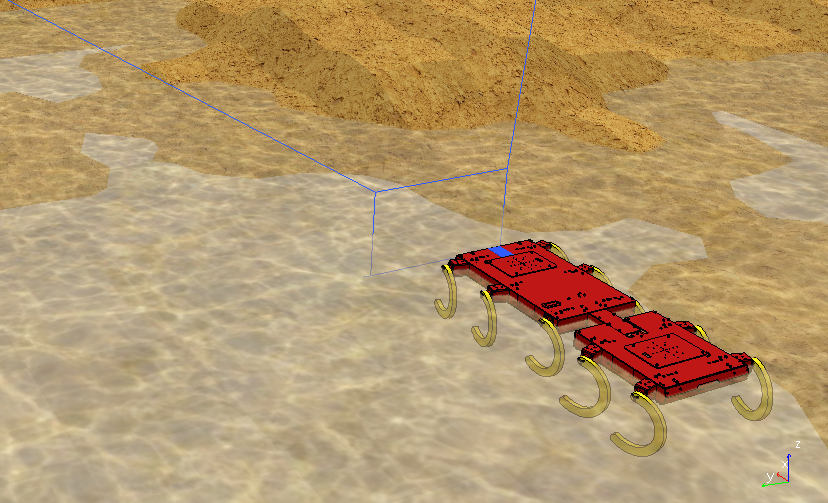
\includegraphics[height=5cm,width=1\textwidth,keepaspectratio]{coppelia_sim.png}
            \caption*{CoppeliaSim симулятор,\\ \textbf{4е поколение} СтриРус}
        \end{subfigure}
        \begin{subfigure}[t]{0.49\textwidth}
            \centering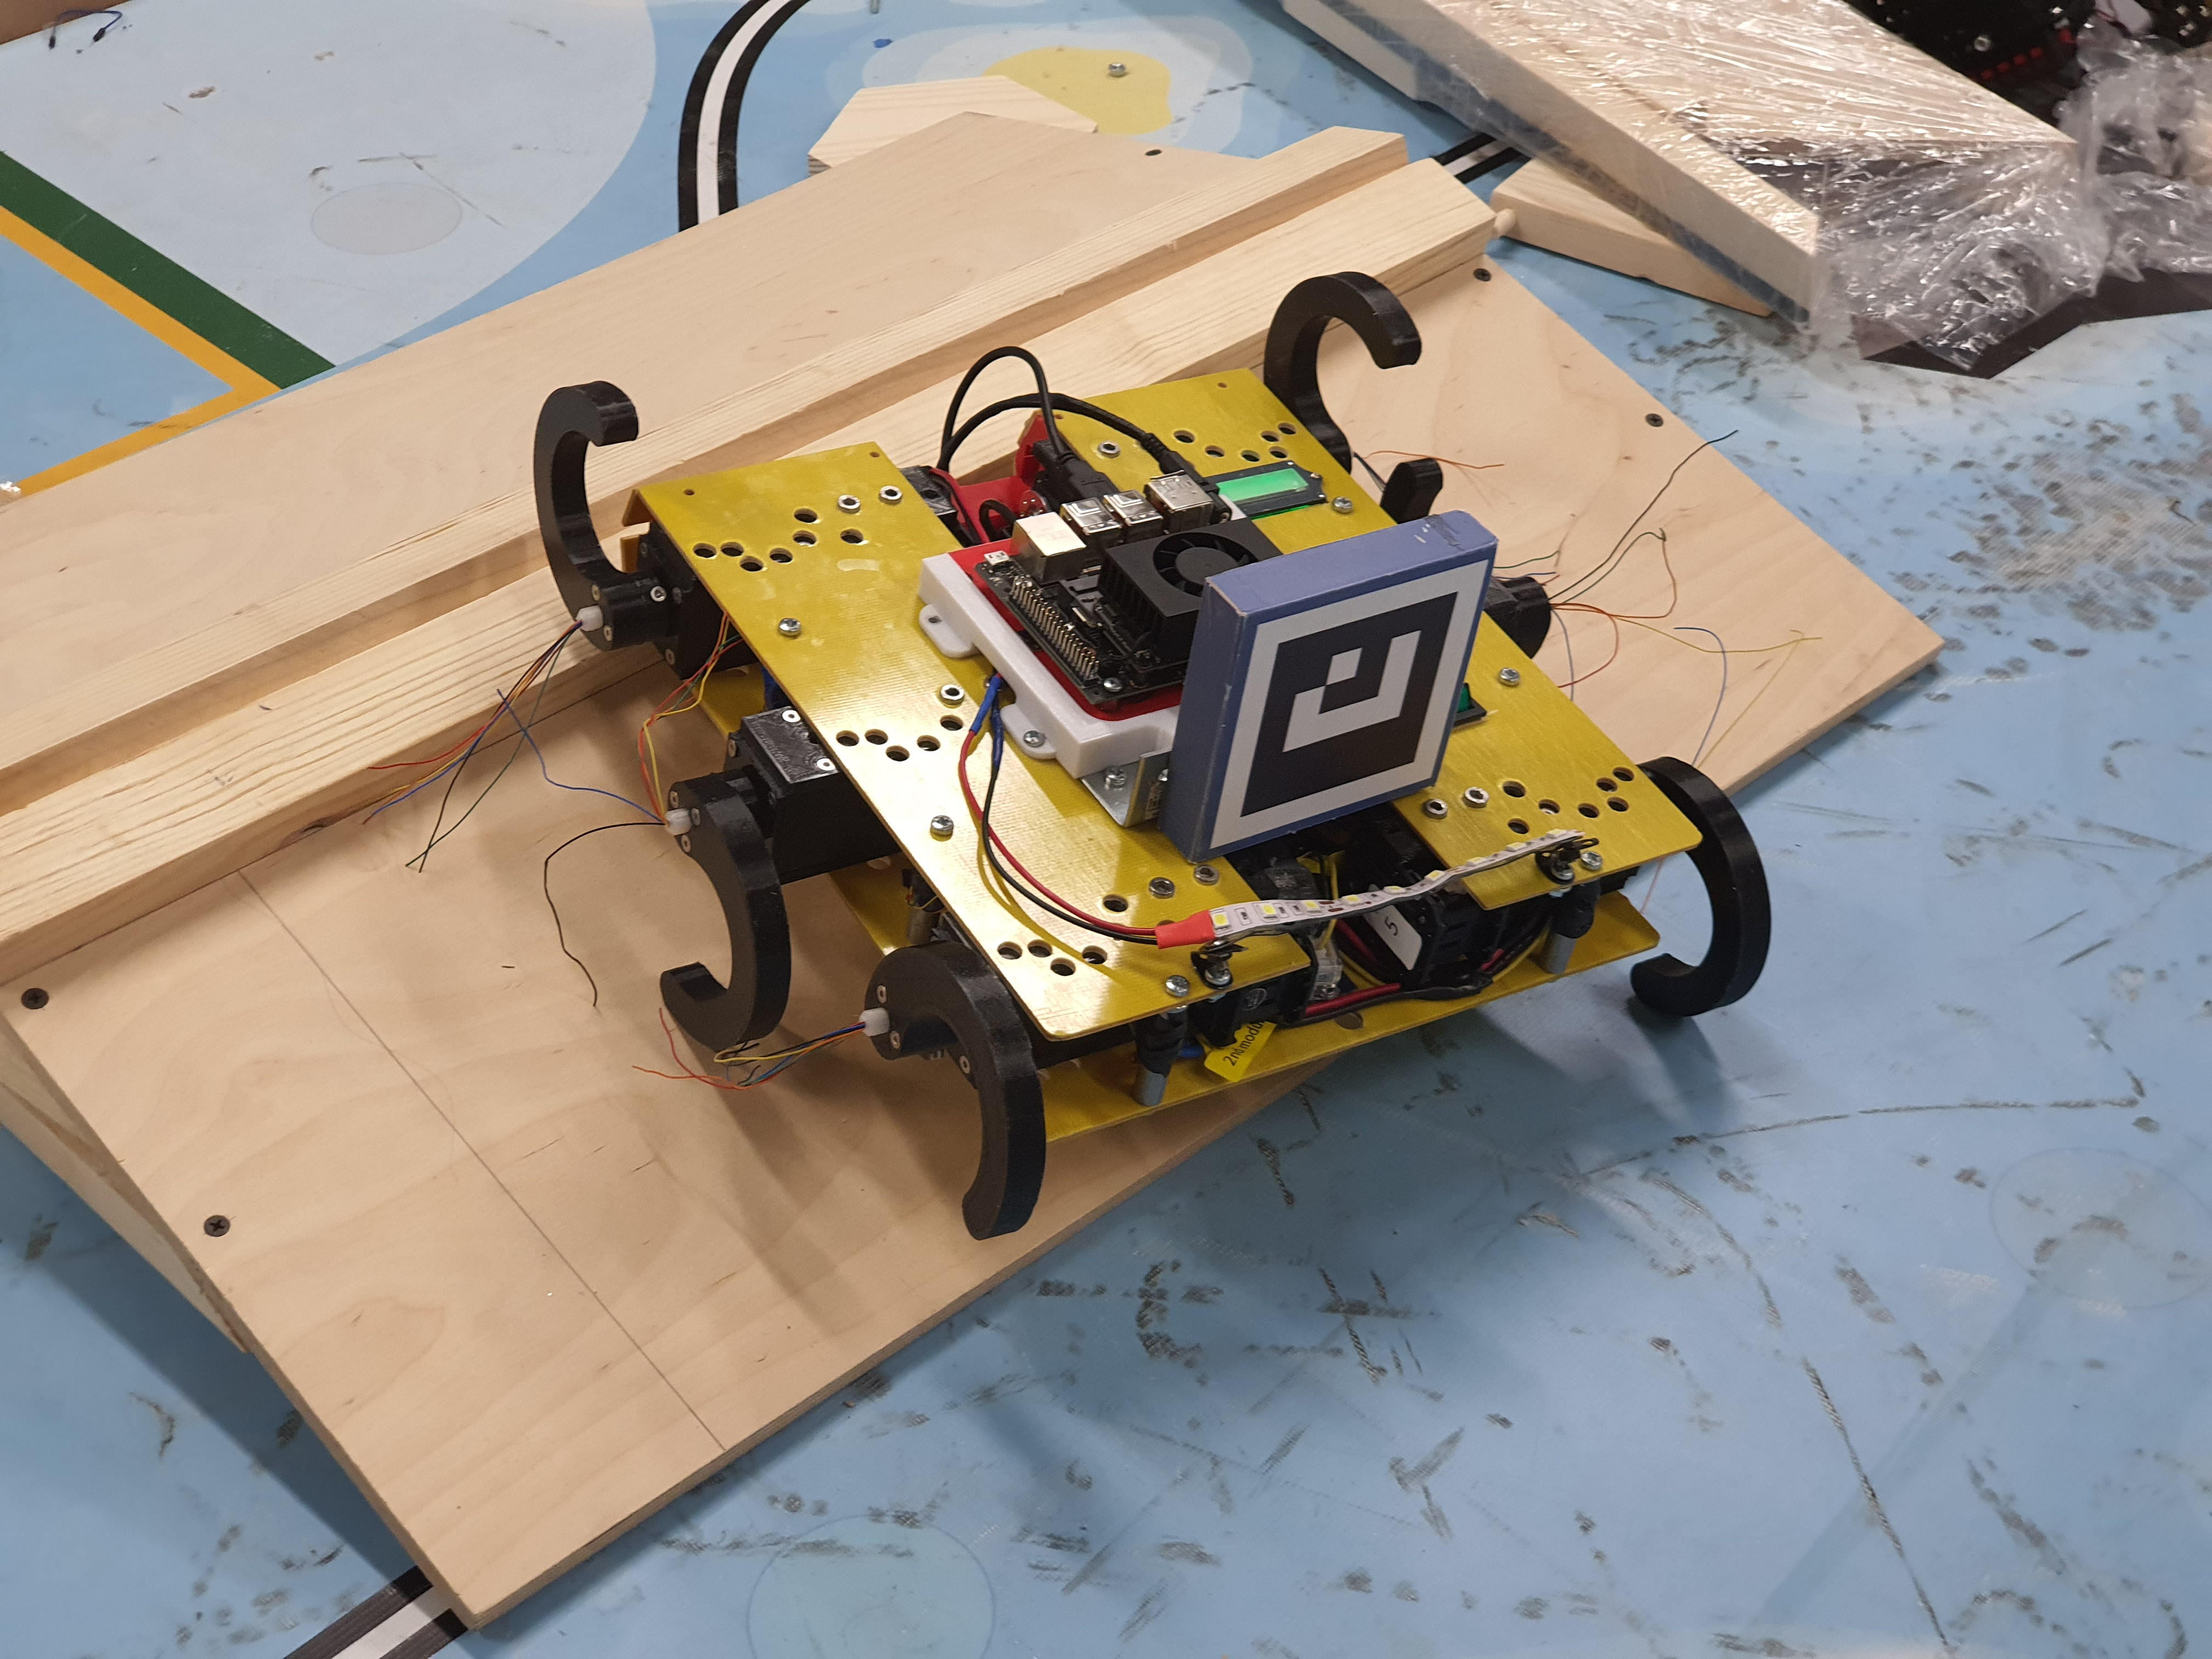
\includegraphics[height=5cm,width=1\textwidth,keepaspectratio]{rl_sim.JPG}
            \caption*{Натурные испытания,\\ \textbf{3е+ поколение} СтриРус}
        \end{subfigure}
    \end{figure}
\end{frame}

\note{\small \setlength{\parindent}{20pt}

Эксперименты проводились как в симуляторе, где использовался последний прототип робота, а также натурно.

Эксперимент выглядел следующим образом. Генерировалось семейство поверхностей и робот ходил с помощью ручного управления определенное время. Полученное облако точек сравнивалось либо с сгенерированным, либо с измеренным в реальной жизни.}

\begin{frame}[t]{Задача локализации}
\framesubtitle{}
\begin{align}
        H_{leg}^{glob} = H(x_{glob},y_{glob},z_{glob},\alpha_{glob},\beta_{glob},\gamma_{glob})T_z(l_1)T_x(l_2)R_y(\alpha_3)T_x(l_4)T_y(l_5)R_z(-15^{\circ})T_y(l_7)R_y(\alpha_8)
\end{align}

\vspace{-0.3cm}
Где $H = \begin{bmatrix}
    \underset{3 \times 3}{R} & \underset{3 \times 1}{T} \\
    \underset{1 \times 3}{0} & \underset{1 \times 1}{1}
\end{bmatrix}$, $R_i$ --- матрица поворота, относительно одной из осей, $T_i$ --- вектор сдвига.

    \begin{columns}[T,onlytextwidth]
        \begin{column}{0.69\textwidth}
            
            \vspace{-0.3cm}
            \begin{figure}[H]
        \centering
        \centering\includegraphics[height=4.5cm,width=1\textwidth,keepaspectratio,page=8]{./tikz_pictures.pdf}
    \end{figure}
        \end{column}
        \begin{column}{0.29\textwidth}
            \begin{figure}[H]
                \centering\includegraphics[height=6cm,width=1\textwidth,keepaspectratio]{../images/slides/snow_local.png}
                \caption{Пример решения задачи локализации с помощью Aruco маркера}
            \end{figure}
        \end{column}
    \end{columns}
\end{frame}

\note{\small \setlength{\parindent}{20pt}

Для решения задачи локализации я решил задачу прямой кинематики для робота *тык*. Таким образом, зная каким сенсором коснулся робот и на какой угол была повернута нога, можно вычислить координату касания опорной поверхности в абсолютной системе координат.

Матрица трансформации от начало абс. системы координаты до робота решалась либо с помощью средств симуляции или с помощью маркеров Аруко, что представлено на картинке *тык*.
}

\begin{frame}[t]{Триангуляция Делоне для вогнутых оболочек}
    \begin{figure}[H]
        \begin{subfigure}[t]{0.3\textwidth}
            \centering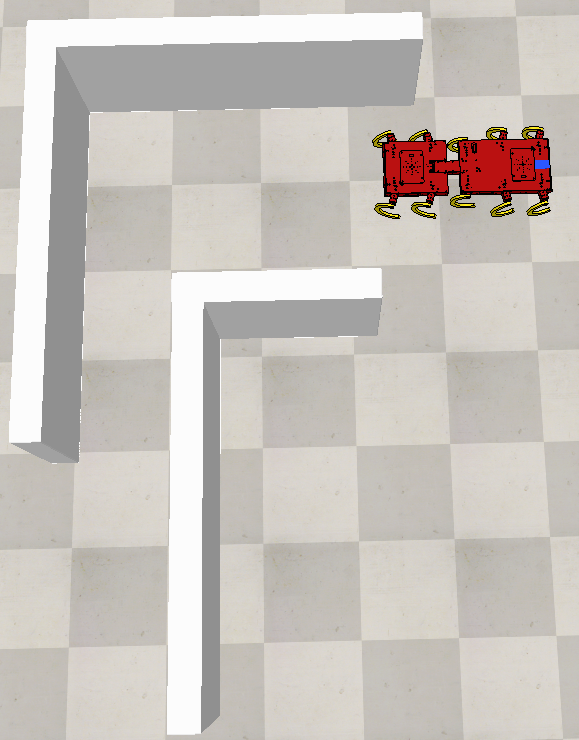
\includegraphics[height=5cm,width=1\textwidth,keepaspectratio]{convex_terr.png}
            \caption*{Пример поверхности}
        \end{subfigure}
        \hfill
        \begin{subfigure}[t]{0.33\textwidth}
            \centering
            \centering\includegraphics[height=6cm,width=1\textwidth,keepaspectratio,page=9]{./tikz_pictures.pdf}
            \caption*{Выпуклая оболочка}
        \end{subfigure}
        \hfill
        \begin{subfigure}[t]{0.33\textwidth}
            \centering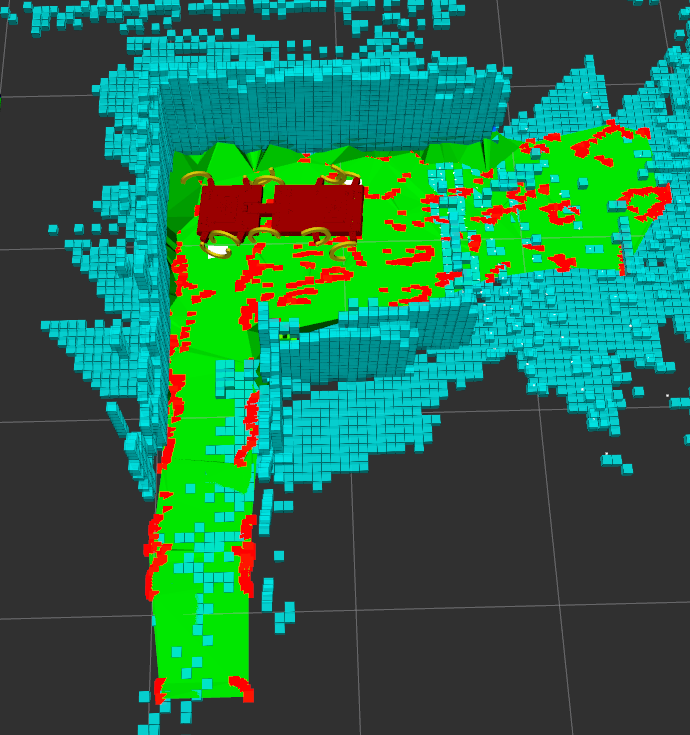
\includegraphics[height=6cm,width=1\textwidth,keepaspectratio]{conv_concave.png}
            \caption*{Вогнутая оболочка}
        \end{subfigure}

    \end{figure}
\end{frame}

\note{\small \setlength{\parindent}{20pt}

Хочется отметить важность использования триангуляции делоне для вогнутых оболочек с помощью данного примера.

Слева картинка поверхности, по которой должне пройти робот *тык*. Отсюда он начал свой путь, здесь он закончил *тык*.

Если мы будем использовать классическую триангуляцию, то получится результат как на рисунке 2 *тык*. Красным отмечена следовая дорожка. Результатом является то, что там где невозможно пройти, карта была все равно построено, что не корректно.

Если же использовать модификацию алгоритма, то будет адекватный результат, как на рисунке справа *тык*}

\begin{frame}[t]{Определение геометрических свойств поверхности}
    \framesubtitle{Результат: Маршрут, полигональная сетка}
    \begin{figure}[H]
        \begin{subfigure}[t]{0.36\textwidth}
            \centering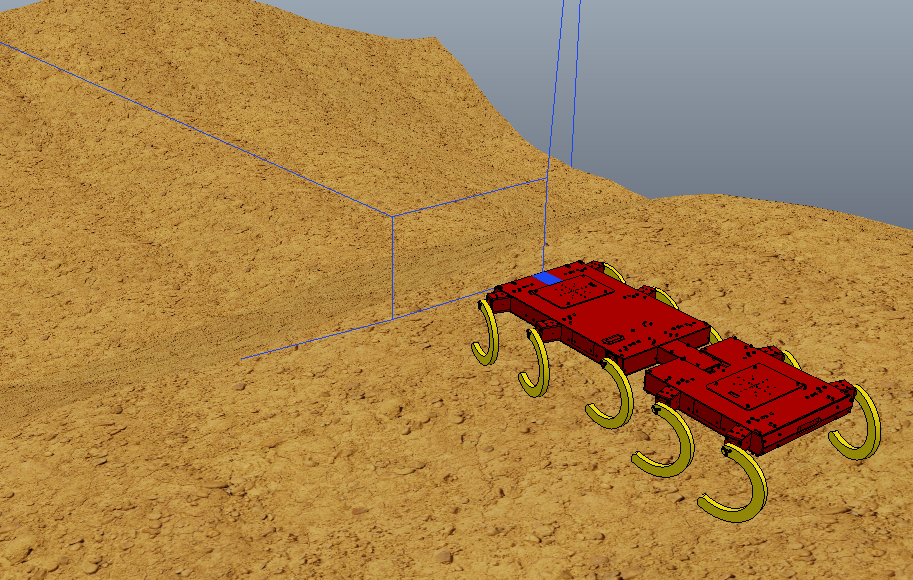
\includegraphics[height=5cm,width=1\textwidth,keepaspectratio]{terrain_wo_water.png}
            \caption*{Начало маршрута}
        \end{subfigure}
        \begin{subfigure}[t]{0.36\textwidth}
            \centering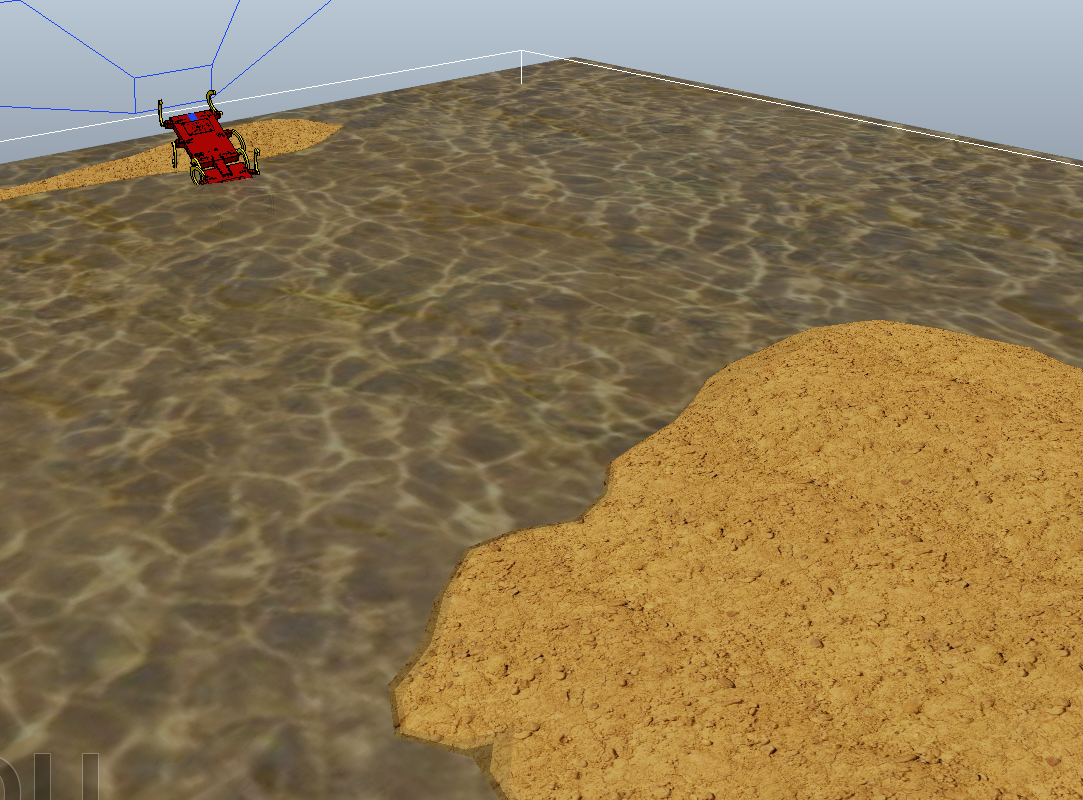
\includegraphics[height=5cm,width=1\textwidth,keepaspectratio]{terrain_w_water_end.png}
            \caption*{Конец маршрута}
        \end{subfigure}
        \begin{subfigure}[t]{0.26\textwidth}
            \centering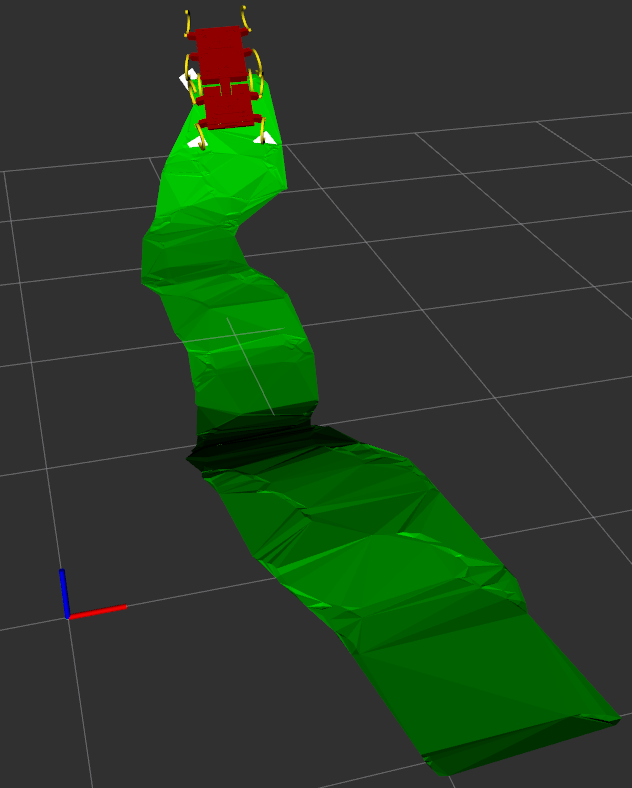
\includegraphics[height=5cm,width=1\textwidth,keepaspectratio]{mesh_rviz.png}
            \caption*{Созданная сетка}
        \end{subfigure}
    \end{figure}
\end{frame}

\note{\small \setlength{\parindent}{20pt}

На слайде представлен один из экспериментов. На рисунках показана поверхность по которой нужно пройти, начало и конец маршрута, а также полученная полигональная сетка *тык, тык и тык*}

\begin{frame}[t]{Определение геометрических свойств поверхности}
    \framesubtitle{Результаты Cloud2Cloud и Cloud2Mesh}
    \begin{figure}[H]
        \begin{subfigure}[t]{0.49\textwidth}
            \centering\includegraphics[height=2.8cm,width=1\textwidth,keepaspectratio,page=10]{./tikz_pictures.pdf}
            % \caption*{Наложенные облака точек}
        \end{subfigure}
        \begin{subfigure}[t]{0.49\textwidth}
            \centering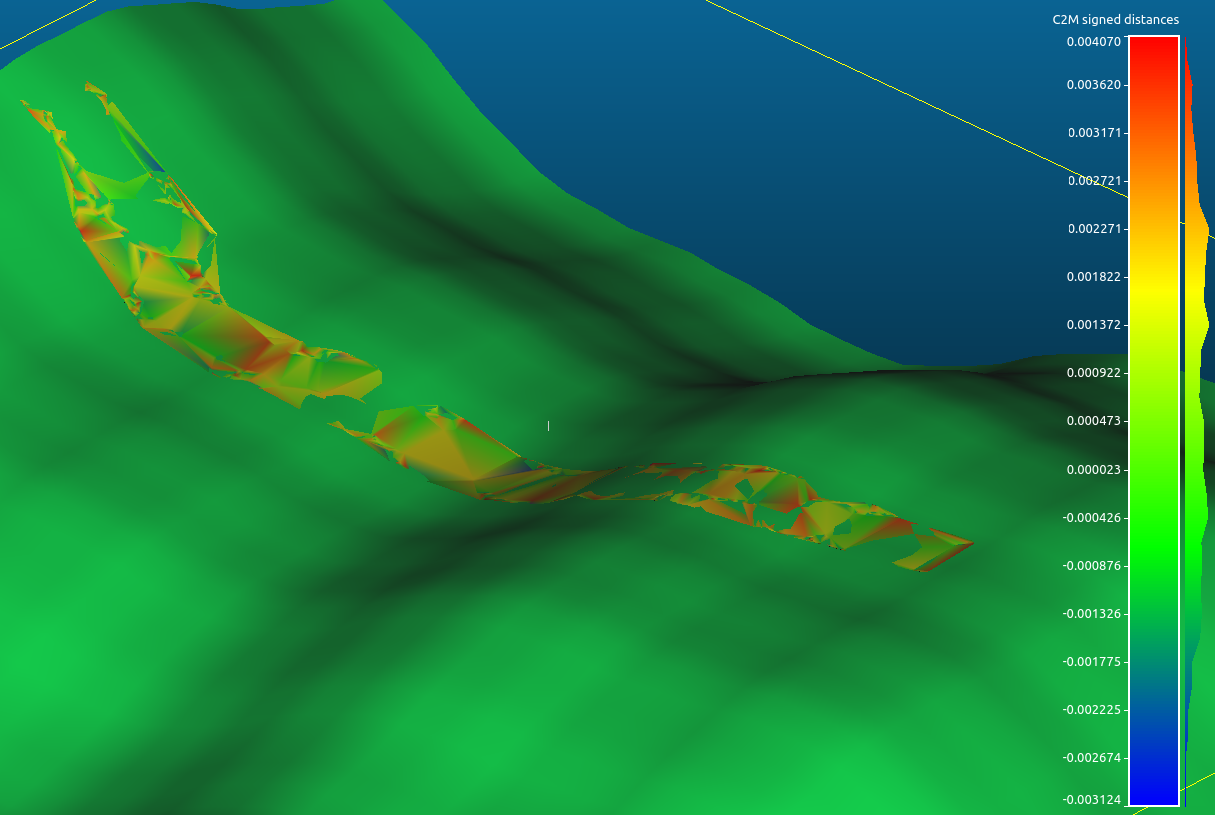
\includegraphics[height=2.8cm,width=1\textwidth,keepaspectratio]{mesh_comp.png}
            % \caption*{Наложенные сетки}
        \end{subfigure}

        \begin{subfigure}[t]{0.49\textwidth}
            \centering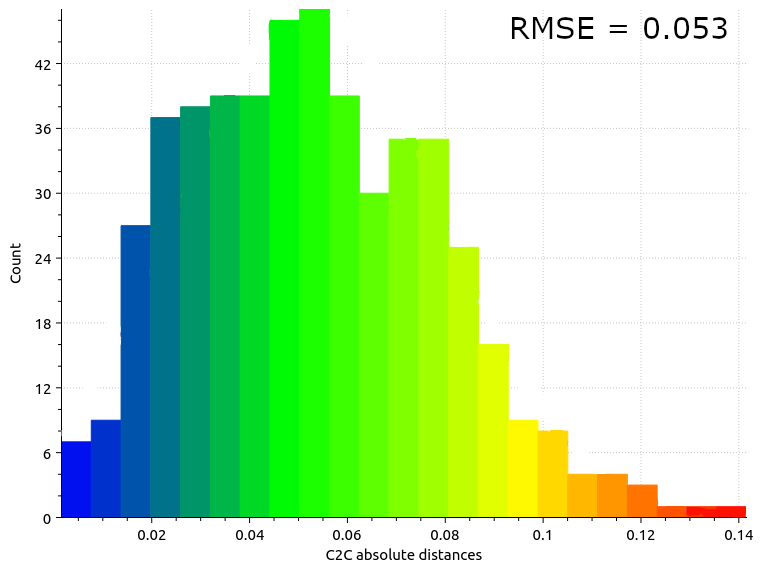
\includegraphics[height=2.6cm,width=1\textwidth,keepaspectratio]{pcd_hist.png}
            \caption*{Гистограмма ошибок C2C}
        \end{subfigure}
        \begin{subfigure}[t]{0.49\textwidth}
            \centering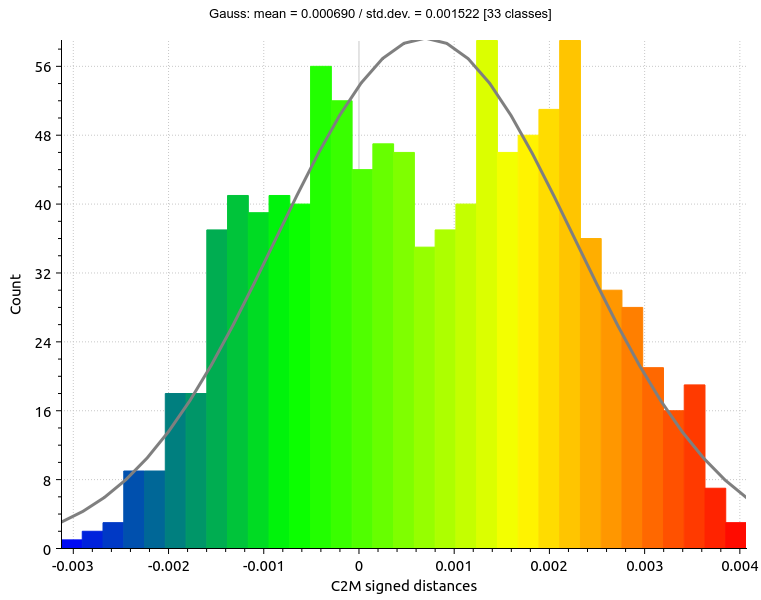
\includegraphics[height=2.6cm,width=1\textwidth,keepaspectratio]{mesh_hist.png}
            \caption*{Гистограмма ошибок C2M}
        \end{subfigure}
    \end{figure}
\end{frame}

\note{\small \setlength{\parindent}{20pt}

Результатами данного эксперимента получились облако точек и полигональная сетка, которые были сравнены с эталонными значениями.

На рисунках представлены гистограммы ошибок двух метрик *тык и тык*, а также наложенные сетки и облака точек *тык и тык*.

Среднеквадратичная ошибка для C2C равна 0.053 метра, а для С2М --- 0.01 м}

\begin{frame}[t]{Определение геометрических свойств поверхности}
    \framesubtitle{Результат: Натурные испытания, Видео}
    \vspace{-0.5cm}
    \begin{figure}[H]
        \begin{subfigure}[t]{0.49\textwidth}
            % \href{run:./videos/big_angle2.mp4}{
            \href{https://youtu.be/2dxHHTG4psQ}{
                \centering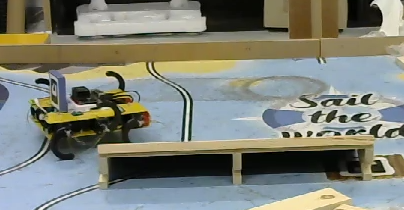
\includegraphics[height=6cm,width=1\textwidth,keepaspectratio]{real_robot_mesh_video_preview.png}}
            \caption*{Робот проходит препятствие}
        \end{subfigure}
        \begin{subfigure}[t]{0.49\textwidth}
            \centering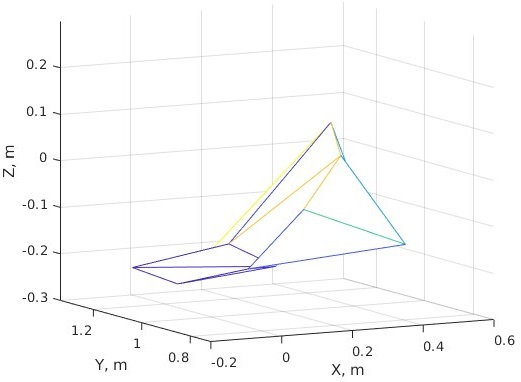
\includegraphics[height=6cm,width=1\textwidth,keepaspectratio]{real_mesh.jpg}
            \caption*{Полигональная сетка, полученная с помощью ног}
        \end{subfigure}
    \end{figure}
\end{frame}

\note{\small \setlength{\parindent}{20pt}

Подобный эксперимент проводился и натурно Слева видео прохождения роботом препятствия *тык*, а также полученная полигональная сетка *тык*. Среднеквадратичная ошибка вышла 0.08 м, что также соответствует допустимой точности.}